\documentclass[a4paper,unicode=true,xetex]{article}
\usepackage{zhfontcfg}
\usepackage{indentfirst}
\usepackage[width=500pt]{geometry}
\usepackage{listings}
\usepackage{color}
\usepackage{graphicx}
\usepackage{tikz}

\renewcommand\figurename{\rm 图}

\setmainfont[BoldFont=YaHei Consolas Hybrid,Mapping=tex-text]{\fontnamesong}
\setsansfont[BoldFont=YaHei Consolas Hybrid,Mapping=tex-text]{\fontnamekai}

\title{Java大作业:图状WordNet浏览器 WNBrowser v1.0}
\author{Y.M.D.项目组}

\begin{document}
\lstset{numbers=none,language=C++,
          frame=trBL,
          breaklines,
          backgroundcolor=\color[rgb]{0.90,0.90,0.90},
          keywordstyle=\color{blue}\bfseries,
          commentstyle=\color{black}, % white comments
          stringstyle=\ttfamily,      % typewriter type for strings
          showstringspaces=false}     % no special string spaces

\fontsize{12pt}{20pt}\selectfont
\maketitle

\noindent{\hei{摘要:}\\
  \kai{
    本实验报告记录了使用JAWS库、JTree以及JGraph \& JGraphT组件开发一个
    WordNet浏览器WNBrowser,以实现对WordNet的图形话表示和查看的过程和
    原理。    
  }
}


\noindent{\hei{关键词:}JAWS,JTree,JGraph,JGraphT,WordNet}

\noindent
\rule{\textwidth}{1pt}
\tableofcontents
\noindent
\rule{\textwidth}{1pt}
\indent

\section{项目名称及目标}

用所学Java知识和提供的数据库,查找资料,实现图形化界面的WordNet。

\section{项目规划及设计}

\subsection{结构规划}

结构总体上分为两大部分:数据接口层,图形显示。这两个部分之间只通过部分的方法接口实现数据传递,可以分开来自由编程实现。

总体的程序流程为:
\begin{enumerate}
\item 用户通过图形界面输入查询单词
\item 图形显示层向数据接口层传送查询单词
\item 数据接口层实现查询单词的检索,以及Cache的维护
\item 数据接口层向图形显示层返回所需数据结果
\item 图形显示层根据所得数据,更新显示页面信息,显示相应查询结果
\end{enumerate}

\subsection{方案设计}

在小组讨论和查找资料过程中,我们Y.M.D.小组设计了两套方案:

\begin{enumerate}
\item 直接使用查询资料所得到的JAWS文件(它们是用Java实现的已打包的数据接口层文件和Cache层文件,只需添加如下语句:import edu.smu.tspell.wordnet.*;并在编译和运行时在classpath中加上 jaws.jar即可),来实现图形界面对所需数据的查询以及对相应数据的解析分类。
\item 通过阅读查询资料所得的上述文件的源码,将整个底层设计简化,模仿学习它们的实现方式,编写我们小组在这个项目中可以使用的简单数据接口层和Cache层,而不考虑过多的程序扩展性。
\end{enumerate}

通过努力,我们最终实现了第一套方案,而第二套方案在具体实现过程中因为简%
化过程涉及面太广,在具体编写过程中遇到很大困难,导致最后只实现了一部分%
功能。

\section{设计分析}

\subsection{数据接口分析}

由结构规划的讨论可知:数据接口层可分为两部分,一个是根据某种条件从文件中查询读取数据部分——数据读取层,另一个则是Cache的维护部分——Cache层。

其中,数据接口层提供两种查询方式:
\begin{enumerate}
\item 根据单词查询,返回相应查询结果;
\item 根据偏移向量信息查询,返回对应文件中该偏移向量信息对应的数据结果。
\end{enumerate}
而Cache层维护两个Cache:
\begin{enumerate}
\item 缓存与当前查询单词有关的各种词性的所有查询结果;
\item 在某一词性条件下,当前查询单词的同义词集中各个词与其在对应文件中的偏移信息。
\end{enumerate}

与此相应的JAWS文件接口分析如下:

(1)数据的存储:

在JAWS文件中,数据的存储结构划分了很多层:

a.定义Synset接口,并在其中定义所有词性下应当实现的返回查询结果的方法

b.对应于各个词性,分别扩展定义与各自词性有关的各个接口:
\begin{lstlisting}

public interface AdjectiveSynset extends Synset

public interface AdjectiveSatelliteSynset extends AdjectiveSynset

public interface AdverbSynset extends Synset

public interface NounSynset extends Synset

public interface VerbSynset extends Synset

\end{lstlisting}
在其中分别定义有关的返回各种数据结果(比如上位词、下位词等)的方法

c.定义抽象类AbstractSynset类,它实现了接口Synset:
\begin{lstlisting}
public abstract class AbstractSynset implements Synset
\end{lstlisting}
d.定义抽象类ReferenceSynset类,它继承了AbstractSynset类

\begin{lstlisting}
public abstract class ReferenceSynset extends AbstractSynset
\end{lstlisting}

e.对应于各个词性,分别扩展定义与各自词性有关的各个子类,并分别实现各自相应的接口:
\begin{lstlisting}
public class AdjectiveReferenceSynset extends ReferenceSynset

implements AdjectiveSynset

public class AdjectiveSatelliteReferenceSynset extends AdjectiveReferenceSynset

implements AdjectiveSatelliteSynset

public class AdverbReferenceSynset extends ReferenceSynset

implements AdverbSynset

public class NounReferenceSynset extends ReferenceSynset

implements NounSynset

public class VerbReferenceSynset extends ReferenceSynset implements VerbSynset
\end{lstlisting}
它们都继承自ReferenceSynset类,并在各自类中定义了与各个词性有关的存储成员变量。

(2)查询接口方法

JAWS文件中为了实现对各个文件的读取和文件中的检索,整个查询接口方法也封装为好几层:

a.定义抽象类WordNetDataBase类,实现最上层的文件读取查询功能,是真个文件读取层的最终封装结果,提供查询方法:
\begin{lstlisting}

public Synset[] getSynsets(String wordForm) throws WordNetException

public Synset[] getSynsets(String wordForm, SynsetType type)

public abstract Synset[] getSynsets(String wordForm, SynsetType type,

boolean useMorphology) throws WordNetException;

public abstract String[] getBaseFormCandidates(String inflection,

SynsetType type);

\end{lstlisting}
以及实例化方法:

\begin{lstlisting}
public synchronized static WordNetDatabase getFileInstance()
\end{lstlisting}

b.定义FileDataBase类,继承自WordNetDataBase类,作为中间的缓冲层,实现更好地扩展功能:

\begin{lstlisting}
public class FileDatabase extends WordNetDatabase
\end{lstlisting}

实际上,WordNetDataBase类提供的实例就是FileDataBase类的实例,该实例可以提供查询方法:

\begin{lstlisting}

public Synset[] getSynsets(String wordForm, SynsetType type,

boolean useMorphology) throws WordNetException

public String[] getBaseFormCandidates(String inflection, SynsetType type)

\end{lstlisting}
在该类的实现中,并不直接实现查询算法和文件的读取。

c.定义WordFormLookup类实现两个Cache的维护以及根据单词查询的查询算法,定义Morphology类返回相应的同义词集Synset中的所有词。

d.定义LineLocator类、MultipleLineLocator类、RandomAccessReader类等类实现文件的检索读取

e.并定义了许多其他的类以实现文件的解析(实在分不清了)。

这样的定义很好地封装了各个类和它们的方法,最上层只需提供简单明了的几个查询方法即可,而且这样的分层很好地保证了各层之间的耦合及扩展,实现了类似“即插即用”的结构。

2、图形显示分析

a.界面总体分析:

在设计的第一阶段,我们准备绘制一个图形界面,将单词的上位词作为按钮呈现在单词的上方,下位词在下方,同义词在左边,反义词在右边,这个方案遇到的主要问题是呈现的位置,因为可能某一个词的上下位不一样多,各种词的词频不同,所以将界面平均分为四份可能会使得一部分太挤,一部分太密;当时的想法是拿一个ScollPane来做,事实上我们最后也是这么做的(使用了JScrollPane)。

在设计的第二阶段,主要是确定了我们界面呈现所采用的数据结构,经过查阅资料,我们惊奇的发现Jgraph在承载我们所需要的要求方面相当的完美,因为Jgraph使用了swing类中的MVC思想,通过传给他一个Model就可以简单的利用其做出非常精美的Graph来,这和我们的初衷是一致的,这一部分的工作主要是由陈志杰同学完成的,在第二阶段的制作过程中,我们一起仔细研究了Jgraph的IDE并做了大量试验,由于是一个全新的内容所以我们在使用它的路上走的非常艰难,10个小时才写出了一百多行的代码,不过在研究的过程中我们基本了解了Jgraph的实现框架,这也为之后的工作打了一个很好的基础。我们最后使用了Jgrapht作为承载Jgraph的Model部分,具体Jgraph的实现可以参考陈部分的报告。在这个阶段我们基本解决了Jgraph的很多问题,并大体建立了界面的几个框架。

图形显示界面如图\ref{fig}所示:
\begin{figure}
  \centering
  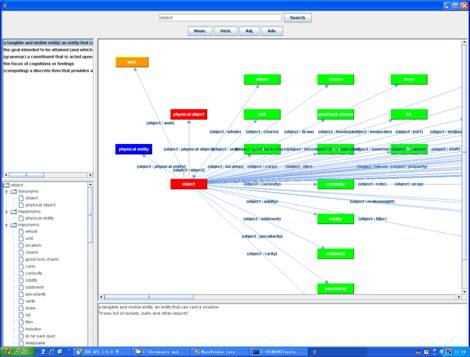
\includegraphics[scale=1.0]{screenshot.jpg}  
  \caption{程序流程图}
  \label{fig}
\end{figure}

整个界面的架构全部使用了javax.swing中的类实现。之所以选择swing包是因为swing包可以更好的兼容Jtree和Jgraph,并且总体来看swing的组件更美观。但是,在实现过程忠,我们也发现swing确实不如awt好用,存在许多漏洞和问题。

我们的整个窗体使用了Jframe,接下来的各个部分主要是使用了JsplitPane来分隔各个组件。窗体的最上方是一个textField,用以输入单词进行查询,下面有四个按钮,分别是对名次,动词,形容词和副词进行查询,窗体的左上角是一个Jlist用以显示选中单词选中意思的解释,当用户输入单词,选中词性再选中一个意思后就得到了一个Synset,可以看作是WordNet网中的一个位置,对应这个位置,会有相关的一些关系,包括上位、下位、派生、近义、反义等等,这些关系主要是通过界面左下方的Jtree和界面右上部的Jgraph来呈现的。在窗体的右下部是一个JTextArea,这个部分主要是用来显示所选Synset的相关意思和用法。

最后一个阶段主要是将想法付诸实施的过程,五个按钮和Jlist单击的事件触发由张宁同学完成,Jgraph的update由陈志杰完成,我完成了剩下的部分,主要包括Jlist的双击事件、JTestArea的呈现、JTree的呈现修改事件处理全部以及界面整体布局的调整和规划。在这一阶段由金鑫大概耗时14小时完成。

在设计触发事件时我们主要通过调用各个组件的Update函数完成,例如修改了Jlist组件的选项,我们需要:
\begin{lstlisting}

UpdateMeaning();

UpdateRelatedWords();

UpdateMeaning();

UpdateJGraph();
\end{lstlisting}
并修改相关的参数。这样做的好处是很多Update的语句可以复用,而且我们只需要控制对其传送的参数(接口)就可以了,方便了编写和调试。

b.Jtree的实现分析

整个过程中最令人头痛的是JTree的部分,以至于花费了将近7个小时的时间在JTree的update上,想起来原理非常简单:在触发了相关的事件后(修改单词、改词性、改解释编号)调用JTree的Update函数完成对Tree的更新。初始的想法是在Update函数中将tree的根节点的所有儿子节点先全部删除,再重建一棵树,并不改变tree与root的链接关系和JsplitPane与tree的链接关系,但事实上出现了非常诡异的现象,就是当查询了一个单词打开JTree后JTree显示正常,但是再查询下一个单词时JTree只有通过改变内容方法得到的root显示的是新单词的内容,而其他子结点部分得到的都是旧的单词的内容。而如果查询了一个新的单词并不打开JTree再查询下一个单词后,那么新单词的JTree则显示正常,这样说明其实JTree的内容是一直随着的单词输入而做出反应得,但是不明白为什么在打开了一次JTree后就出现了问题,通过很多方法进行调试但是也没有发现问题所在,最后怀疑是内部的机制所致。于是决定换一种方法,经过一个试验小程序的调试发现必须将JTree也整个new一个并加到一个new出来的组件再将这个new出来的组件加到原来的大组件上才能得到正确的结果。于是我们决定就这么做。但是问题又来了,我的承载JTree的组件是JSplitPane,如果new一个JSplitPane那么这个new出口的JsplitPane就和整个Frame脱节了,所以需要层层new,层层add,最后通过这个巧妙的方法解决了问题。整个过程耗时7个小时之多,但是很高兴最后解决了它,也在研究过程中对swing的组件有了更深刻的认识。

最后就是JTree事件的处理,值得一提的是在界面组件的所有双击事件都没有相应的事件处理函数,但是有一个通用的方法,就是可以通过鼠标事件进行处理:

例如
\begin{lstlisting}
tree.addMouseListener(new MouseAdapter()

{

private long clickTime;

public void mouseReleased(MouseEvent me)

{

if (checkClickTime())

{

//What you want to do in this Action write here. ^_^

}

}

public boolean checkClickTime()

{

long nowTime = (new Date()).getTime();

if (nowTime - clickTime < 300)

{

clickTime = nowTime;

return true;

}

clickTime = nowTime;

return false;

}

});
\end{lstlisting}

c.JGraph的实现分析:

JGraph是一个纯Java开发的图形组件,支持拖,放,缩放,合并等其它操作。它可以被结合到任何的Swing应用程序当中。它分为Free、Pro和Layout Pro版本,我们实际使用的是他的Free版本。

JGraph的画图机制:

JGraph将图元定义为一个一个的cell,每个cell可以是一个顶点(Vertex)、边(Edge)或者节点(Port中的一种。顶点可以有邻接的顶点,他们通过边相联系,边联接的两个端点称为目标和源,每个目标或者源是一个节点。节点是顶点的孩子。每个cell都可以有自己的孩子。

顶点(Vertex)对应的类为org.jgraph.graph.DefaultGraphCell

边(Edge)对应的类为org.jgraph.graph.DefaultEdge

节点(Port)对应的类为org.jgraph.graph.DefaultPort

每个cell的外观由相应的属性定义,属性序列是指一系列的键-值对,他们以Map形式组织(实际实现中使用的是AttributeMap),例如:

//修改某个节点的位置
\begin{lstlisting}
private void positionVertexAt( Object vertex, int x, int y ) {

DefaultGraphCell cell = grpAdapter.getVertexCell(vertex);

AttributeMap attr = cell.getAttributes();

GraphConstants.setBounds( attr, new Rectangle( x, y, 100, 30 ) );

cell.setAttributes(attr);

}

//修改模个节点的颜色

private void setVertexColor( Object vertex, Color color ) {

DefaultGraphCell cell = grpAdapter.getVertexCell(vertex);

AttributeMap attr = cell.getAttributes();

GraphConstants.setBackground(attr, color);

cell.setAttributes(attr);

}
\end{lstlisting}
JGraph只是提供单纯的图形绘制功能,不包含实际的数据,所以要想办法把自己的数据加进去才行,这恐怕就得考虑扩展JGraph了,我们在参照比较了网上各种对于JGraph的抽象,最终确定使用一个名字为JGraphT的第三方组件。

JGraph的扩展——JGraphT

JGraphT是对于图数据的抽象,可以很方便的建立起各种有向图和无向图的逻辑结构,通过一个GraphAdapter可以实现与JGraph的对接,进而将逻辑的图结构借助JGraph显示出来。不过对于MVC中的V(View)和C(Control),即图的具体显示方式,节点位置、颜色之类的,还是要通过调用JGraph的方法来实现。如上个例子,即是先通过JGraphT中的方法获得某节点在JGraph中的对应对象后,再通过修改这个对应对象来达到改变颜色和位置的目的的。

四、心得

虽然制作时间不多,但得到了非常好的效果,特别是使用了协同开发工具%
subversion之后,工作效率很高。同时在编写大作业的过程中我们也查阅了大量%
的资料,学习了很多课本以外的知识,获益匪浅!


\section{项目组成员}

\subsection{成员组成及联系方式}
\begin{itemize}
\item 陈志杰 00648333 TEL: 13581738579  chenzhijie@icst.pku.edu.cn
\item 金鑫 superjinxin@pku.edu.cn
\item 袁文清 00648231 ywq8876@163.com
\item 张宁 00648179 eighteenzhang@sohu.com
\end{itemize}

\subsection{成员分工情况}

\begin{itemize}
\item 陈志杰:资料搜集,JGraph操作部分,文件读取器的Cache部分(未完成)。
  工作量 25\%。
\item 金鑫:资料搜集,JTree操作部分,JGraph前期实验。工作量 25\%。
\item 袁文清:资料搜集,文件读取器底层部分(未完成),项目报告文档。工
  作量 25\%。
\item 张宁:界面中除去JGraph和JTree的其他部分,源程序注释。工作量 25\%。
\end{itemize}


\end{document}
%%% Local Variables: 
%%% mode: latex
%%% TeX-master: t
%%% End: 
